\chapter{Hashfunktionen}\label{cha:hash}
\section{Grundlagen}
Hashfunktionen\indexHashFunction sind Funktionen, die von einer großen,
potentiell unbeschränkten, Menge in eine kleinere Menge abbilden. Also 
\begin{align*}
H_k\colon \{0,1\}^* \rightarrow \{0,1\}^k\, ,
\end{align*}
wobei $k$ den in \ref{sec:secparam} eingeführten Sicherheitsparameter
bezeichnet.  Diese Funktionen werden dazu verwendet, größere Datenmengen
effizient zu kennzeichnen (ihnen sozusagen einen Fingerabdruck
zuzuordnen). Die Anwendungsgebiete für Hashfunktionen in der Informatik
sind vielfältig, wir werden uns aber in diesem Skript auf ihre
kryptographischen Anwendungen beschränken\indexCryptHashFunction.

\section{Sicherheitseigenschaften}
Um eine Hashfunktion im kryptographischen Sinne\indexCryptHashFunction
verwenden zu können, reicht eine Funktion, die von einer großen Menge in
eine kleine Menge abbildet, nicht aus. 
Sie muss zusätzlich einige weitere Anforderungen erfüllen.

\subsection{Kollisionsresistenz}
Die wichtigste Eigenschaft einer Hashfunktion $H$ ist die
Kollisionsresistenz (\emph{collision
  resistance})\indexCollisionResistance. Das bedeutet, es soll schwierig
sein, zwei unterschiedliche Urbilder $X, X'$ zu finden, für die gilt: 
\begin{align*}
X \neq X' \text{ und } H(X) = H(X')
\end{align*}

Da wir von einer großen in eine kleine Menge abbilden, kann $H$ nicht
injektiv sein. Es ist uns also nicht möglich, Kollisionen komplett zu
verhindern. Trotzdem können wir fordern, dass diese möglichst selten
auftreten. Präziser formuliert verlangen wir, dass bei jeder
kollisionsresistenten Hashfunktion ein PPT Algorithmus eine Kollision
nur mit im Sicherheitsparameter $k$ vernachlässigbarer
Wahrscheinlichkeit findet.
\begin{definition}[Kollisionsresistenz]
Eine Funktion $H_k$ ist kollisionsresistent\indexCollisionResistance,
wenn jeder PPT-Algorithmus nur mit höchstens in $k$ vernachlässigbarer
Wahrscheinlichkeit eine Kollision findet.  Präziser formuliert ist der
Vorteil für jeden PPT-Angreifer $\A$
\begin{align*}
Adv^{cr}_{H,\A}(k)\coloneqq \Pr \left[ (X, X') \leftarrow \A(1^k) : X \neq X'
  \land H_k(X) = H_k(X')\right] 
\end{align*}
in $k$ vernachlässigbar.
\end{definition}

\subsection{Einwegeigenschaft}
Die zweite kryptographisch wichtige Eigenschaft von Hashfunktionen ist
die Einwegeigenschaft (\emph{pre-image
resistance})\indexPreImageResistance, die sicherstellt, dass eine
Hashfunktion nur in eine Richtung berechenbar ist. Genauer gesagt
fordern wir, dass es bei einem gegebenen Wert $H(X)$ \emph{schwierig}
ist, ein passendes $X$ zu finden.

Es stellt sich nun die Frage, wie eine Hashfunktion beschaffen sein
muss, damit sie die Einwegeigenschaft erfüllen kann. Ist z.B. die
Urbildmenge zu klein, kann durch Raten einfach auf ein passendes $X'$
geschlossen werden. Außerdem sollte es intuitiv keinen Kandidaten $X'$
als Urbild für $H(X)$ geben, der wahrscheinlicher ist als andere
Kandidaten. Um das zu erreichen, wird für die Elemente der Urbildmenge
üblicherweise eine Gleichverteilung angestrebt.

\begin{definition}[Einwegfunktion]
Eine über $k$ parametrisierte Funktion $H$ ist eine Einwegfunktion
\indexPreImageResistance bezüglich der Urbildverteilung $\chi_k$, wenn
jeder PPT-Algorithmus nur mit höchstens in $k$ vernachlässigbarer
Wahrscheinlichkeit ein Urbild eines gegebenen, aus $\chi_k$ bezogenen
Bildes findet. Genauer ist der Vorteil für jeden PPT-Angreifer $\A$
\begin{equation*}
Adv^{ow}_{H,\A}(k)\coloneqq \Pr \left[ X' \leftarrow \A(H(X), 1^k) : H(X) = H(X')\right]
\end{equation*} 
in $k$ vernachlässigbar, wobei $X \leftarrow \chi_k$ gewählt
wurde. Dabei muss $\A$ nicht zwingend $X' = X$ zurückgeben.
\end{definition}

Die Forderungen nach Kollisionsresistenz und Einwegeigenschaft, die wir
bisher für eine kryptographische Hashfunktion aufgestellt haben, hängen
bei näherer Betrachtung sehr eng miteinander
zusammen\indexCollisionResistance\indexPreImageResistance. Das führt uns
zu folgender Feststellung:

\begin{theorem}
Jede kollisionsresistente Hashfunktion $H_k \colon \{0,1\}^* \rightarrow
\{0,1\}^k$ ist eine Einwegfunktion bzgl. der Gleichverteilung auf
$\{0,1\}^{2k}$. 
\end{theorem}

\begin{beweisidee}
$H_k$ hat $2^k$ Bilder und $2^{2k}$ Urbilder. Es gibt also weniger als
$2^k$ Nachrichten, die auf einen Hashwert abgebildet werden, der genau einer
Nachricht zugeordnet werden kann. Es hat also bei $X \in \{0,1\}^{2k}$ fast jedes
Urbild $X$ viele "`Nachbarn"' $X'$ mit $H(X) = H(X')$, denn für die
Wahrscheinlichkeit, dass ein Element $H(X)$ der Bildmenge nur ein
einziges Urbild $X$ besitzt, gilt

\begin{equation*}
\Pr \left[ | H^{-1}(H(X))| = 1\right] \leq \frac{2^k}{2^{2k}} = \frac{1}{2^k}.
\end{equation*}
Die Wahrscheinlichkeit ist also vernachlässigbar im Sicherheitsparameter
$k$.
\end{beweisidee}

\begin{beweis}
Zu jedem $H$-Invertierer $\A$ geben wir nun einen $H$-Kollisionsfinder $\B$ an mit
\begin{equation*}
Adv^{cr}_{H,\B}(k) \geq \frac{1}{2} \cdot Adv^{ow}_{H,\A}(k) - \frac{1}{2^{k+1}}
\end{equation*} 
Nun wählt $\B$ ein $X \leftarrow \{0,1\}^{2k}$ gleichverteilt zufällig
und gibt $H(X)$ als Eingabe an $\A$. $\B$ setzt nun $X' \leftarrow
\A(1^k, H(X))$ und gibt $(X, X')$ aus. Dann gilt für $\B$s
Erfolgswahrscheinlichkeit:
\begin{align*}
	&\Pr \left[\B \text{ gewinnt}\right]\\
	&= \Pr\left[H(X) = H(X') \land X \not = X'\right]\\
	&= \Pr \left[\A \text{ invertiert} \land X \not = X'\right]\\
	&\geq \Pr \left[\A \text{ invertiert} \land X \not = X' \land \vert H^{-1}(H(X)) \vert > 1\right]\\
	&= \underbrace{\Pr \left[X \not = X' \biggm| \A \text{ invertiert} \land \vert H^{-1}(H(X)) \vert > 1\right]}_{\geq \frac{1}{2}}
	\cdot \underbrace{\Pr \left[\A \text{ invertiert} \land \vert H^{-1}(H(X)) \vert > 1\right]}_{\geq \Pr \left[\A \text{ invertiert}\right] - \frac{1}{2^k}}\\
	&\geq \frac{1}{2} \cdot Adv^{ow}_{H,\A}(k) - \frac{1}{2^{k+1}}
\end{align*}
\qed
\end{beweis}


\subsection{Target Collision Resistance}
Die \emph{Target Collision Resistance}\indexTargetCollisionResistance
(auch \emph{second pre-image resistance} oder \emph{universal one-way})
ist eine weitere Eigenschaft, die zur Bewertung von Hashfunktionen
herangezogen wird. Genügt eine Hashfunktion $H$ der Target Collision
Resistance, ist es \textit{schwierig}, für ein gegebenes Urbild $X$ ein
$X' \not = X$ zu finden, für das gilt: $H(X') = H(X)$.

Die Target Collision Resistance stellt einen Zwischenschritt zwischen
Kollisionsresistenz und Einwegeigenschaft dar: Kollisionsresistenz
impliziert die Target Collision Resistance, welche wiederum die
Einwegeigenschaft impliziert. Formal ergibt sich:

\begin{definition}[Target Collision Resistance]
Eine über $k$ parametrisierte Funktion $H$ genügt der Target Collision
Resistance\indexTargetCollisionResistance, falls für jeden PPT-Angreifer
$\A$ bei gegebenem, zufällig gezogenem $X$ die Wahrscheinlichkeit
\begin{equation*}
Adv^{tcr}_{H,\A}(k)\coloneqq \Pr \left[ X' \leftarrow \A(X, 1^k) : X \neq X'
  \land H_k(X) = H_k(X')\right] 
\end{equation*}
in $k$ vernachlässigbar ist.
\end{definition}
\subsection{Beispiele}

\begin{beispiel}[Kollisionsresistenz bei Signaturverfahren]\indexCollisionResistance
Eve und Bob beschließen, gemeinsam online Verträge abzuschließen. Hierzu
verwenden sie ein \textit{Hash-then-Sign}-Verfahren, dass in Kapitel
\ref{subsec:hash-then-sign} noch näher betrachtet wird. Wir können uns
das Verfahren wie 
folgt vorstellen: 
\begin{enumerate}
\item Eve sendet eine Nachricht an Bob.
\item Bob berechnet den Hashwert und erstellt kryptographische
  Signatur (eine Art \glqq elektronische Unterschrift\grqq, siehe
  Kapitel \ref{cha:symauth}) für diesen Hashwert.
\item Bob sendet diese Signatur an Eve
\item Eve berechnet eine eigene Signatur für die Nachricht. Nun kann Eve
  anderen gegenüber beweisen, dass sie und Bob dem Inhalt der Nachricht
  zustimmen. 
\end{enumerate}
Ist die Hashfunktion nun nicht kollisionsresistent, ist folgender
Angriff möglich:
\begin{enumerate}
\item Eve erstellt zwei Verträge $\plaint_1$ und $\plaint_2$ mit
  $H(\plaint_1) = H(\plaint_2)$, wobei
  $\plaint_1$ ein fairer Vertrag und $\plaint_2$ ein unfairer Vertrag
  ist, dem Bob niemals zustimmen würde.
\item Eve sendet $\plaint_1$ an Bob. Bob stimmt dem Vertrag zu und
  sendet Eve deshalb seine Signatur für $H(\plaint_1)$.
\item Eve benutzt diese Signatur, um gegenüber anderen vorzuweisen, dass
  Bob dem Vertrag $\plaint_2$ zugestimmt hat.
\end{enumerate}
\end{beispiel}

\begin{beispiel}[Einweg-Eigenschaft beim Speichern von Passwörtern]\indexPreImageResistance
Angewendet werden Hashes beispielsweise beim Speichern von
Passwörtern auf einem Server. Der Server speichert nur $H(X)$ ab und
vergleicht bei einem Anmeldungsversuch lediglich $H(X)$ mit dem ihm vom
Client zugesendeten $H(X')$. Dadurch muss das Passwort nicht im Klartext
auf dem Server liegen. Wie wir in Kapitel~\ref{cha11} sehen werden, gibt
es aber effiziente Angriffsmöglichkeiten, weswegen heutzutage neben dem
Hash des Passworts auch noch ein \emph{Salt} gespeichert wird, der
zufällig für jedes Passwort generiert wird.
Die Einwegeigenschaft der Hashfunktion stellt sicher, dass ein
Angreifer, der in Besitz der Liste der Passwort-Hashes kommt, aus
diesen keine Passwörter berechnen kann.
\end{beispiel}

\begin{beispiel}[Target-Kollisionsresistenz in der Computer-Forensik]\indexTargetCollisionResistance
Eine Anwendung von kryptographischen Hashfunktionen ist die
Computer-Forensik. Hierbei wird, z.B. zur Verbrechensermittlung, eine
Festplatte auf bestimmte Dateien hin untersucht. Da man sich den Aufwand
ersparen möchte, alle Dateien händisch zu untersuchen, geht man wie
folgt vor:
\begin{enumerate}
  \item Erstelle eine Whitelist, die für bekannte, gutartige
    Dateien(z.B. Bestandteile des Betriebssystems) die Hashwerte
    enthält, sowie ein Blacklist für entsprechend bösartige Dateien.
  \item Untersuche diejenigen Dateien, die auf keiner der beiden Listen
    genannt sind, genauer.
\end{enumerate}

Wenn die verwendete Hash-Funktion nun nicht target-kollisionsresistent
ist, kann dies verwendet werden, um bösartige Dateien zu
verstecken. Angenommen, ein Terrorist möchte die Datei
\texttt{bombenbauanleitung.pdf} so speichern, dass sie im Falle einer
Beschlagnamung des Computers nicht entdeckt wird. Er benennt sie deshalb
um in \texttt{betriebsanleitung.pdf}. Außerdem bricht er die
Target-Kollisionsresistenz und verändert seine Datei so, dass ihr Hash
mit dem der Betriebsanleitung des Betriebssystems übereinstimmt. Diese
wird mit großer Wahrscheinlichkeit auf der Whitelist der Polizei
stehen. Deshalb wird sie bei einer Untersuchung nicht
auffallen\cite{Stevens2012}.
\end{beispiel}
\section{Merkle-Damgård-Transformation}
\label{ch:hash:merkledamgard}
In der Praxis werden Hashfunktionen benötigt, die nicht nur die
Eigenschaften aus den obigen Abschnitten berücksichtigen, sondern auch
flexibel in ihrer Eingabelänge und konstant in ihrer Ausgabelänge
sind. Typischerweise werden für diesen Zweck
\emph{Merkle-Damgård-Transformation} eingesetzt.

\subsection{Struktur von Merkle-Damgård}
Die Eingabenachricht wird bei einer Merkle-Damgård-Transformation
\indexMDTransformation $H_{\textnormal{MD}}$ zunächst in Blöcke
$\plaint_{1},\dots, \plaint_{n}$ mit fester Blocklänge $l$ aufgeteilt.
Auf diese Blöcke wird anschließend nacheinander eine
Kompressionsfunktion $F \colon \{0, 1\}^{l + k} \rightarrow \{0,1\}^{k}$
angewendet, die %die Blöcke mithilfe eines Eingabeparameters $Z$ auf
eine festgelegte Länge die Blöcke auf eine feste Länge $k \leq l$
verkürzt.

Aus dem ersten Nachrichtenblock $\plaint_{1}$ und dem
Initialisierungsvektor $IV \in \{0, 1\}^k$ wird durch die
Kompressionsfunktion ein Bitstrom $Z_1$ der Länge $k$ berechnet, der mit
Hilfe von $\plaint_2$ zu $Z_2$ berechnet wird. Diese Berechnung setzen
wir analog für die restlichen Nachrichtenblöcke fort und erhalten mit
$Z_{n}$ den Hashwert für die Nachricht. Formal dargestellt erhalten wir:
\begin{align*}
  Z_0 &= IV\\
  \forall i \in \{1,\dots, n\}\colon Z_{i} &= F(Z_{i-1} \concat M_{i})
\end{align*}
Der Ablauf ist schematisch in Abbildung~\ref{fig:md-konstruktion} gezeigt.

Der Initialisierungsvektor $IV$\indexIV wird dabei für jede
Hashfunktion fest gewählt. Aus Sicherheitsgründen ist es, wie wir in
Beweis~\ref{md-proof} sehen werden, notwendig, die Nachrichtenlänge an
das Ende der Nachricht anzuhängen. Falls es im letzten Block nicht
genügend freie Bits gibt, wird diese an das Ende eines neuen Blocks
geschrieben. Die übrigen Bits werden gepaddet.

%Ist der letzte Block $M_{n}$ zu kurz, wird er auf die benötigte
%Blocklänge gepaddet.  
%Das Padding enthält dabei die Nachrichtenlänge, um zu verhindern, dass
%Verlängerungen der Nachricht für einen Angriff genutzt werden können.
\begin{figure}[h]
  \begin{center}
    \unitlength=1mm
    \linethickness{0.4pt}
    \begin{picture}(110,20)

      \put(5,5){\vector(1,0){15}}
      \put(12,6){\makebox(0,0)[cb]{IV}}

      \put(25,15){\vector(0,-1){7.5}}
      \put(28,10){\makebox(0,0)[cb]{$M_1$}}

      \put(20,2.5){\framebox(10,5){$F$}}

      \put(30,5){\vector(1,0){12}}
      \put(36,6){\makebox(0,0)[cb]{$Z_1$}}

      \put(47,15){\vector(0,-1){7.5}}
      \put(50,10){\makebox(0,0)[cb]{$M_2$}}

      \put(42,2.5){\framebox(10,5){$F$}}

      \put(52,5){\vector(1,0){12}}
      \put(58,6){\makebox(0,0)[cb]{$Z_2$}}

      \put(68,4){\makebox(0,0)[cb]{\ldots}}

      \put(72,5){\vector(1,0){12}}
      \put(78,6){\makebox(0,0)[cb]{$Z_{n-1}$}}

      \put(84,2.5){\framebox(10,5){$F$}}

      \put(89,15){\vector(0,-1){7.5}}
      \put(92,10){\makebox(0,0)[cb]{$M_{n}$}}

      \put(94,5){\vector(1,0){12}}
      \put(100,6){\makebox(0,0)[cb]{$Z_{n}$}}

    \end{picture}
  \end{center}
  \caption{Merkle-Damgård-Transformation $H_{\textnormal{MD}}$}
  \label{fig:md-konstruktion}
\end{figure}

\subsection{Sicherheitseigenschaften der Merkle-Damgård-Transformation}
Die Sicherheit einer Merkle-Damgård-Transformation
\indexMDTransformation $H_{\textnormal{MD}}$ hängt stark von der
verwendeten Kompressionsfunktion $F$ ab: 
\begin{theorem}
Ist $F$ kollisionsresistent, so ist auch $H_{\textnormal{MD}}$ kollisionsresistent.
\end{theorem}

\begin{beweis}\label{md-proof}
Gegeben sei zwei Nachrichten $M \neq M'$ mit $H_{\textnormal{MD}}(M) =
H_{\textnormal{MD}}(M')$. Wir führen diese Kollision nun auf eine
Kollision in $F$ zurück. Da es eine Kollision in $H_{\textnormal{MD}}$
gibt, gilt $Z_{n} = F(Z_{n-1} \concat M_{n}) = F(Z'_{n-1} \concat
M'_{n}) = Z'_{n}$. 
\begin{description}
\item[Fall 1:] $Z_{n-1} \neq Z'_{n-1}$ oder $M_{n} \neq M'_{n}$
  $\Rightarrow$ Es wurde eine Kollision in $F$ gefunden.  
\item[Fall 2:] $Z_{n-1} = F(Z_{n-2} \concat M_{n-1}) = F(Z'_{n-2}
  \concat M'_{n-1}) = Z'_{n-1}$ $\Rightarrow$ Wir überprüfen analog
  beide Fälle für die Bitstrings $Z_{n-2} \concat M_{n-1}$ und $Z'_{n-2}
  \concat M'_{n-1}$. 
\end{description}
Wir überprüfen beide Fälle für alle Argumente $Z_{i-1} \concat M_{i}$,
$Z'_{i-1} \concat M'_{i}$ $(1 \leq i \leq n)$, bis wir eine Kollision in
$F$ gefunden haben. Da nach Voraussetzung $M \neq M'$ gilt und die
Nachrichtenlängen angehängt wurden, gibt es mindestens ein $M_{i} \neq
M'_{i}$ und damit eine Kollision in $F$.  Hätten wir also einen
Angreifer, der effizient Kollisionen für $H_\textnormal{MD}$ findet,
könnten wir daraus einen Angreifer konstruieren, der effizient
Kollisionen für $F$ berechnet, was im Widerspruch zur angenommenen
Kollisionsresistenz von $F$ steht.
\qed
\end{beweis}

\subsection{Bedeutung von Merkle-Damgård}
\subsubsection{Secure Hash Algorithm (SHA)}
Im Jahr 1995 veröffentlichte die NIST den von der NSA entworfenen, auf
der Merkle-Damgård-Transformation beruhenden, kryptographischen
Hashalgorithmus \emph{Secure Hash Algorithm 1} (SHA-1)\indexSHAOne
\cite{NIST_SHA95}. Lange Zeit war SHA-1 die wichtigste kryptographische
Hashfunktion, bis der Algorithmus im Jahr 2005 zumindest theoretisch
gebrochen wurde. Es existieren also Angriffe, die schneller als eine
Brute-Force-Suche sind, eine explizite Kollision wurde bislang
allerdings nicht gefunden. In Folge des Bekanntwerdens der
Schwachstellen empfiehlt die NIST auf die Verwendung von SHA-1 zu
verzichten. Dennoch hat SHA-1 wenig von seiner Verbreitung eingebüßt und
wird heutzutage immer noch weitreichend verwendet, z.B. bei Prüfsummen.

\paragraph*{Ablauf des Hash-Vorgangs}

\begin{enumerate}
\item Teile die Nachricht in $n$ 512-Bit große Blöcke $\plaint_{1},\dots,\plaint_{n}$ auf und padde den letzten Block bei Bedarf.
\item Initialisiere $H_0^{(0)}, \dots, H_4^{(0)}$ mit fest gewählten Konstanten und setze $a = H_0^{(0)}, \dots, e = H_4^{(0)}$.
\item Für alle Nachrichtenblöcke $\plaint_{i}$ von $i = 1,\dots,n$:
  \begin{enumerate}
  \item Führe 80 Berechnungsrunden $t = 0,\dots,79$ aus, um die neuen Hashwerte für $a,\dots,e$ zu bestimmen.	
    \begin{figure}[h]
      \centering
      \tikzstyle{every circle node}= [draw]
      \begin{tikzpicture}
        \begin{scope}[>=latex] %for filled arrow tips
          \newcommand{\n}{5}
          
          \pgfmathsetmacro\minBoxWidth{(2.0)} // 2.2 old
          \pgfmathsetmacro\minBoxHeight{(0.6)} // 0.5 old
          
          \pgfmathsetmacro\xA{int(0)}
          \pgfmathsetmacro\xB{(\minBoxWidth * 1)}
          \pgfmathsetmacro\xC{(\minBoxWidth * 2)}
          \pgfmathsetmacro\xD{(\minBoxWidth * 3)}
          \pgfmathsetmacro\xE{(\minBoxWidth * 4)}
          
          \node (h0) at (\xA, {(\n -1)*2 + 2}) [draw,thick,minimum width=\minBoxWidth cm, minimum height=\minBoxHeight cm] {$H_0^{(i-1)}$};
          \node (h1) at (\xB, {(\n -1)*2 + 2}) [draw,thick,minimum width=\minBoxWidth cm, minimum height=\minBoxHeight cm] {$H_1^{(i-1)}$};
          \node (h2) at (\xC, {(\n -1)*2 + 2}) [draw,thick,minimum width=\minBoxWidth cm, minimum height=\minBoxHeight cm] {$H_2^{(i-1)}$};
          \node (h3) at (\xD, {(\n -1)*2 + 2}) [draw,thick,minimum width=\minBoxWidth cm, minimum height=\minBoxHeight cm] {$H_3^{(i-1)}$};
          \node (h4) at (\xE, {(\n -1)*2 + 2}) [draw,thick,minimum width=\minBoxWidth cm, minimum height=\minBoxHeight cm] {$H_4^{(i-1)}$};
          
          \pgfmathsetmacro\abcdeLineYCoord{(\n -1)*2 + 0.9}
          
          \node (a) at (\xA, \abcdeLineYCoord) [draw,thick,minimum width=\minBoxWidth cm, minimum height=\minBoxHeight cm] {$a$};
          \node (b) at (\xB, \abcdeLineYCoord) [draw,thick,minimum width=\minBoxWidth cm, minimum height=\minBoxHeight cm] {$b$};
          \node (c) at (\xC, \abcdeLineYCoord) [draw,thick,minimum width=\minBoxWidth cm, minimum height=\minBoxHeight cm] {$c$};
          \node (d) at (\xD, \abcdeLineYCoord) [draw,thick,minimum width=\minBoxWidth cm, minimum height=\minBoxHeight cm] {$d$};
          \node (e) at (\xE, \abcdeLineYCoord) [draw,thick,minimum width=\minBoxWidth cm, minimum height=\minBoxHeight cm] {$e$};
          
          \draw[->,semithick] (h0) -- (a);
          \draw[->,semithick] (h1) -- (b);
          \draw[->,semithick] (h2) -- (c);
          \draw[->,semithick] (h3) -- (d);
          \draw[->,semithick] (h4) -- (e);
          
          \pgfmathsetmacro\numAddBoxes{int(4)}
          \pgfmathsetmacro\lastAddBoxIndex{int(\numAddBoxes)}
          \pgfmathsetmacro\firstAddBoxYCoord{\abcdeLineYCoord - 1.5}
          
          % \node (plus0)[circle, draw] at (\xE,\firstAddBoxYCoord) {$+$};
          
          \foreach \nr in {1, ..., \numAddBoxes}{
            \node (plus\nr)[circle] at (\xE,{\abcdeLineYCoord - (1.5 * \nr)}) {$+$};
          }	
          
          \pgfmathsetmacro\lastAddBoxYCoord{\abcdeLineYCoord - 1.5 * \numAddBoxes}
          \draw[->,semithick] (e) -- (plus1);
          
          \foreach \nr in {1, ..., 3}{
            \pgfmathsetmacro\cnr{int(\nr + 1)}
            \draw[->,semithick] (plus\nr) -- (plus\cnr);
          }
          
          % draw Key and Message arrow
          \node (KeyArrow) at (\xE + 2.0, {\abcdeLineYCoord - (1.5 * 2)}) {$K_t$};
          \draw[->, semithick] (KeyArrow) -- (plus2);
          
          \node (MessageArrow) at (\xE + 2.0, {\abcdeLineYCoord - (1.5 * 4)}) {$W_t$};
          \draw[->, semithick] (MessageArrow) -- (plus4);
          
          \node (shiftL5)[ellipse, draw] at (\minBoxWidth * 0.5 + 0.1, \firstAddBoxYCoord) {$<< 5$};
          
          \node (p1)[circle, fill, inner sep=0cm, minimum size=0.12cm] at (\xA, \firstAddBoxYCoord) {};
          \draw[->, semithick] (p1) -- (shiftL5);
          \draw[->, semithick] (shiftL5) -- (plus1);
          
          \node (shiftR2)[ellipse, draw] at (\xB, \lastAddBoxYCoord) {$>> 2$};
          \draw[->, semithick] (b) -- (shiftR2);
          
          \node (rectF)[draw,thick,rounded corners,minimum width=0.6cm, minimum height=2.1cm] at (\xD + 0.7, {\abcdeLineYCoord - (1.5 * 3)}) {$F_{t}$};
          \node (p2)[circle, fill, inner sep=0cm, minimum size=0.12cm] at (\xC, {\abcdeLineYCoord - (1.5 * 3)}) {};
          \draw[->, semithick] (p2) |- (rectF);
          \draw[->, semithick] (rectF) -- (plus3);
          
          \node (p3)[circle, fill, inner sep=0cm, minimum size=0.12cm] at (\xB, {\abcdeLineYCoord - (1.5 * 3) + 0.5}) {};
          \draw[->, semithick] (p3) -- ($(rectF) + (-0.3, 0.5)$);
          
          \node (p4)[circle, fill, inner sep=0cm, minimum size=0.12cm] at (\xD, {\abcdeLineYCoord - (1.5 * 3) - 0.5}) {};
          \draw[->, semithick] (p4) -- ($(rectF) + (-0.3, -0.5)$);
          
          
          \node (aNew) at (\xA, {\lastAddBoxYCoord - 2.5}) [draw,thick,minimum width=\minBoxWidth cm, minimum height=\minBoxHeight cm] {$a$};
          \node (bNew) at (\xB, {\lastAddBoxYCoord - 2.5}) [draw,thick,minimum width=\minBoxWidth cm, minimum height=\minBoxHeight cm] {$b$};
          \node (cNew) at (\xC, {\lastAddBoxYCoord - 2.5}) [draw,thick,minimum width=\minBoxWidth cm, minimum height=\minBoxHeight cm] {$c$};
          \node (dNew) at (\xD, {\lastAddBoxYCoord - 2.5}) [draw,thick,minimum width=\minBoxWidth cm, minimum height=\minBoxHeight cm] {$d$};
          \node (eNew) at (\xE, {\lastAddBoxYCoord - 2.5}) [draw,thick,minimum width=\minBoxWidth cm, minimum height=\minBoxHeight cm] {$e$};
          % \draw[->, semithick] (shiftL5) -- (plus1);
          
          \draw[->, semithick] (a) -- (\xA, {\lastAddBoxYCoord - 1.0}) 
          -- (\xB, {\lastAddBoxYCoord - 1.5}) -- (bNew);
          
          \draw[->, semithick] (shiftR2) -- ($(shiftR2) + (0, -1)$) 
          -- (\xC, {\lastAddBoxYCoord - 1.5}) -- (cNew);
          
          \draw[->, semithick] (c) -- (\xC, {\lastAddBoxYCoord - 1.0}) 
          -- (\xD, {\lastAddBoxYCoord - 1.5}) -- (dNew);
          
          \draw[->, semithick] (d) -- (\xD, {\lastAddBoxYCoord- 1.0}) 
          -- (\xE, {\lastAddBoxYCoord - 1.5}) -- (eNew);
          
          \draw[->, semithick] (plus\lastAddBoxIndex) -- (\xE, {\lastAddBoxYCoord- 0.7}) 
          -- (\xA, {\lastAddBoxYCoord - 1.5}) -- (aNew);
          
          \node (AddModText) at (\xE - 1.4, {\lastAddBoxYCoord - 3.0}) {\scriptsize{Addition ist modulo $2^{32}$ zu verstehen}};
          
        \end{scope}
      \end{tikzpicture}
      \caption{Schema der Berechnungsrunde}
    \end{figure}
  \item Setze $H_0^{(i)} = H_0^{(i-1)} + a, \dots, H_4^{(i)} = H_4^{(i-1)} + e$.
  \end{enumerate}
\item Gebe $H_0^{(n)} \concat \dots \concat H_4^{(n)}$ als 160-Bit
  Hashwert (\emph{message digest}) aus. 
\end{enumerate} 

In jeder der 80 Berechnungsrunden zum Berechnen eines
Zwischenergebnisses werden folgende Funktionen, Konstanten und Variablen
verwendet: 
\begin{itemize}
\item Rundenfunktion $F_{t}$ führt, je nach Index, unterschiedliche
  Elementaroperationen auf den 32-Bit langen Variablen $b, c, d$ aus.
\item Konstante $K_{t}$ hat, je nach Index, vier verschiedene Werte.
\item Variable $W_{t}$, als \emph{message schedule} bezeichnet, besteht
  in den ersten 16 Runden jeweils aus einem 32-Bit Wort des aktuellen
  512-Bit großen Nachrichtenblocks $\plaint_{i}$ und in den
  verbleibenden 64 Runden aus einem rekursiv berechneten Wert
  vergangener message schedules des gleichen Blocks.
\end{itemize}

Für die Eingangs erwähnten Angriffe auf die beschriebene Konstruktion
wird die Möglichkeit ausgenutzt, für eine Runde Kollisionen zu finden
und versucht, diese auf mehrere Runden auszuweiten. Dabei sind auch
ähnliche Ausgaben hilfreich. Der schnellste der im Jahr 2005
vorgestellten Algorithmen benötigt mit ungefähr $2^{63}$-Schritten
(vgl. $2^{80}$-Schritte für einen Brute-Force-Angriff) zwar noch immer
einen beträchtlichen Rechenbedarf, erzeugt jedoch Kollisionen über alle
80 Berechnungsrunden.

Neben SHA-1 ist der im Jahr 1992 von Ronald Rivest veröffentlichte
MD5-Algorithmus\indexMDFive eine bekannte Hashfunktion, die auf dem
Merkle-Damgård-Konstrukt beruht und für eine Vielzahl kryptographischer
Anwendungen und Datenintegritäts-Sicherung eingesetzt wurde. Von der
Verwendung von MD5 sollte für sicherheitsrelevante Anwendungsszenarien
mittlerweile jedoch abgesehen werden: Im Unterschied zu SHA-1 können bei
MD5 explizite Kollisionen gefunden werden. Im Jahr 2013 stellten Xie
Tao, Fanbao Liu und Dengguo Feng den bis dato besten Angriff vor, der
aus einer Menge von etwa $2^{18}$ MD5 Hashwerten ein Kollisionspaar
findet. Heutige Prozessoren benötigen dafür weniger als eine Sekunde.
%fact check mit Hofheinz

Aufgrund der Verwundbarkeit von MD5 und SHA-1 empfiehlt die NIST
heutzutage mindestens eine Hashfunktion der SHA-2-Familie\indexSHATwo
zu verwenden. Ähnlich zu SHA-1 basieren die Funktionen dieser
Hash-Familie auf der Merkle-Damgård-Konstruktion, bieten jedoch in der
Praxis, aufgrund des größeren Bildraums, ein höheres Maß an
Sicherheit. Theoretisch aber bleiben die Funktionen, wegen großen
Ähnlichkeiten in der Konstruktion, verwundbar. Deshalb wurde im Jahr
2013 mit SHA-3\indexSHAThree (\glqq Keccak\grqq{}-Algorithmus) der
Versuch gestartet, eine grundlegend andere kryptographische Hashfunktion
zu standardisieren, die keine Merkle-Damgård-Konstruktion
verwendet. Dieser Standardisierungsprozess wurde am 05.08.2015 mit der
Veröffentlichung des NIST\footnote{Das Abschlussdokument findet sich
unter
\url{https://www.federalregister.gov/articles/2015/08/05/2015-19181/announcing-approval-of-federal-information-processing-standard-fips-202-sha-3-standard}}
abgeschlossen\footnote{Die Übersicht über den Standardisierungsprozess
findet sich auf
\url{http://csrc.nist.gov/groups/ST/hash/sha-3/sha-3_standardization.html}.}.


\section{Angriffe auf Hashfunktionen}
\subsection{Birthday-Attack}\indexBirthDayAttack
Für diesen Angriff berechnen wir möglichst viele $Y_i = H(X_i)$.
Danach suchen wir unter diesen Hashwerten nach Gleichheit (und finden so
$X \not = X'$ mit $H(X) = Y = Y' = H(X')$). 
\paragraph*{Vorgehen:}
\begin{enumerate}
  \item Schreibe $(X_i, Y_i)$ in Liste. Dabei ist $X_i \in \{0,1\}^{2k}$
    gleichverteilt und $Y_i = H(X_i)$.  
  \item Sortiere die Liste nach $Y_i$.
  \item Untersuche die Liste auf $Y_i$-Kollisionen.
\end{enumerate}

\begin{theorem}
Sei $n \leq 2^{\frac{k}{2}}$ und $Y_1, \ldots , Y_n \in \{0,1\}^k$
unabhängig gleichverteilt. Dann gibt es $i \not = j$ mit $Y_i = Y_j$ mit
Wahrscheinlichkeit $p > \frac{1}{11} \cdot \frac{n^2}{2^k}$.
\end{theorem}
\begin{beweis}
  ohne Beweis
\end{beweis}
Wir haben also schon für $n = 2^{\frac{k}{2}}$ zufällige, verschiedene
$X_i$ mit einer Wahrscheinlichkeit von $p > \frac{1}{11}$ Kollisionen
unter den den dazugehörigen $Y_i$. Für die Berechnung brauchen wir
$\Theta(k \cdot 2^{\frac{k}{2}})$ Schritte und haben einen
Speicherbedarf von $\Theta(k \cdot 2^{\frac{k}{2}})$ Bits.

\subsection{Weitere Angriffe}
Auch ein Meet-in-the-Middle-Angriff\indexMeetInTheMiddle kann die Zeit
zum Auffinden einer Kollision verkürzen. Allerdings setzt dieser Angriff
voraus, dass die Hashfunktion eine "`Rückwärtsberechnung"' zulässt.
\paragraph*{Angriffsbeschreibung}
\begin{itemize}
\item Gegeben: $M = (M_1,\dots,M_n), H(M), i$.
\item Gesucht: $M' = (M'_1,\dots,M'_n) \neq M$, so dass $H(M') = H(M)$.
  \begin{enumerate}
  \item Teile $M$ in Substrings $P = (M_1,\dots,M_i)$ und $S = (M_{i+1},\dots,M_{n})$.
  \item Berechne für jedes $P' = (M'_1,\dots,M'_i)$ den Wert $Z = H(P')$.
  \item Sortiere die Liste aller $Z$, um binäre Suche zu ermöglichen.
  \item Rechne ausgehend von $H(M)$ für ein $S' =
    (M'_{i+1},\dots,M'_{n})$ zu $Z'$ zurück. 
    \begin{enumerate}
    \item Falls $Z'$ in der Liste aller $Z$ enthalten ist und das
      entsprechende $P' \neq P$ oder $S' \neq S$, dann haben wir eine
      Kollision für $M$ mit $M' = P' \concat S'$ gefunden. 
    \item Wiederhole den Schritt ansonsten für ein anderes $S'$.
    \end{enumerate}
  \end{enumerate}
\end{itemize}
Der Aufwand für diesen Angriff nähert sich asymptotisch dem für die
Geburtstagsattacke an. 

\begin{figure}[h]
  \centering
  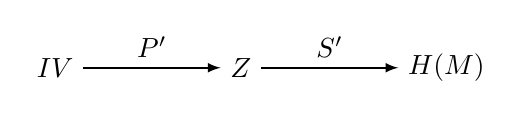
\begin{tikzpicture}[>=latex]		
    \node[anchor=east] (IV) at (0, 0) {$IV$};
    \node (Z) at (2, 0) {$Z$};
    \node[anchor=west] (H) at (4, 0) {$H(M)$};
    
    \draw[->, semithick] (IV.east) -- (Z.west) node[above, pos=.5]{$P'$};
    \draw[->, semithick] (Z.east) -- (H.west) node[above, pos=.5]{$S'$}; 
  \end{tikzpicture}
  \caption{Hilfsskizze für Meet-in-the-Middle-Angriff auf eine Hashfunktion $H$}
  \label{fig:md-meet-in-the-middle-attack}
\end{figure}
\subsection{Fazit}
Die vorgestellten Angriffe zeigen, dass sich der Aufwand zum Finden
einer Kollision gegenüber einer Brute-Force-Attacke stark verringern
lässt. Bei einer Hash-Ausgabe mit einer Länge $\geq k$ Bits kann man nur
mit einer "`Sicherheit"' von $\frac{k}{2}$ Bits rechnen.

%%% Local Variables:
%%% mode: latex
%%% TeX-master: "skript"
%%% End:
